\title{Babascript: }

\etitle{Babascript: }

\author{匿名で査読を行うため著者名なし
  \affil{匿名で査読を行うため所属名なし}}

\begin{abstract}

プログラムに人への処理命令を組み込むことのできるプログラミングフレームワーク Babascript を提案する。
人をコンピュータやセンサーのような、タスクを処理するためのノードとして扱うことによって、タスクを処理する上で人とコンピュータに対して最適な処理を割り当て、人とコンピュータがお互いの得意なことを実行し、目的を達成できるような環境を実現する。
また、Babascriptフレームワークによって実現する応用例を示し、起こりうる問題について考察する。


\end{abstract}

\maketitle

\section{はじめに}\label{ux306fux3058ux3081ux306b}

プログラムはコンピュータの挙動を制御するためのものとして存在してきた。
近年は実世界の要素の挙動を制御する用途としても利用されるようになってきた。
しかし、未だに実世界の主な構成要素たる人間の挙動を制御することはできていない。
まだ書けてない

\section{Babascript
プログラミング環境}\label{babascript-ux30d7ux30edux30b0ux30e9ux30dfux30f3ux30b0ux74b0ux5883}

Babascript環境では関数呼び出しによって人に命令を送る仕組みによって、プログラム内での人への処理命令を実現する。
通常のプログラムでは、関数に引数を与え実行することで、処理結果を返り値として得ることができる。
Babascriptでは、同様に関数呼び出しし、処理を人に実行させ、返り値を処理結果として返す。
つまり、同じ関数呼び出しだが、その実行主体を人間にすることによって、プログラム内における人力処理の組み込みを実現する。

このような仕組みを実現するために、人への命令構文を組み込んだライブラリ
Babascript と、命令に対して返り値を返すためのクライアントライブラリ
Babascript
Client、クライアントライブラリを組み込んだWebアプリケーションを実装した、
また、プラグイン機構によってその機能を拡張可能にした。

\begin{figure}[h]
  \centering
  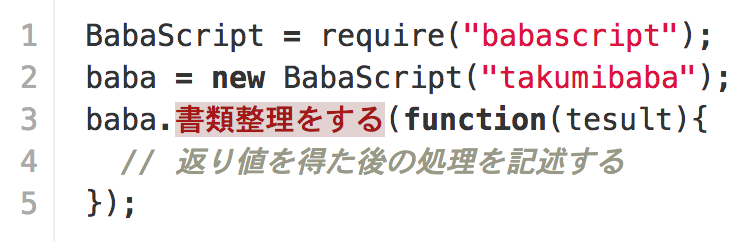
\includegraphics[width=220px]{./images/script_01.png}
  \caption{babascriptプログラムの基本命令文}
  \label{script_01}
\end{figure}

\subsection{BabaScript}\label{babascript}

Babascriptは、関数呼び出しによって人に処理命令を送れるオブジェクト(以下、人オブジェクト)を宣言可能にするDSLだ。
人オブジェクトにおいて定義されていない全てのメソッドが人への命令として解釈される。
また、命令に対して人からの返り値を得ると、実行メソッドの引数で指定したコールバック関数を実行する。

\subsubsection{人オブジェクトの宣言と処理命令構文}\label{ux4ebaux30aaux30d6ux30b8ux30a7ux30afux30c8ux306eux5ba3ux8a00ux3068ux51e6ux7406ux547dux4ee4ux69cbux6587}

図\ref{script_01}のようなプログラムによって、人に処理命令を送ることができる。
メソッド名がそのまま命令内容となる。

人への命令構文は、実行されるとメソッド名と引数を元にしたjsonオブジェクトへと変換され、このjsonオブジェクトが処理タスクとしてクライアントライブラリに配信される。

人オブジェクトは宣言時にIDを指定することによって、誰に対して処理命令を配信するかを決定する。
例えば、id:baba
に命令を送りたければ、人オブジェクト宣言時の第一引数にはbabaという文字列を指定する必要がある。
また、クライアント側でも同様に、id:baba として宣言する必要がある。

この際、指定したIDを監視するクライアントが複数人だった場合は、人への命令構文を実行時に他のタスクを実行していないクライアントへタスクが配信される。

人への処理命令構文の第一引数には基本的な処理情報に加えてクライアント側に送信するオプション情報を指定し、第二引数には、人から処理命令に対する返り値が得られた際に実行するコールバック関数を指定する。
コールバック関数実行時には、その引数に返り値と関連した情報を格納したオブジェクトが与えられる。

オブジェクトに定義されていない全ての関数は人への処理命令構文として解釈される。
この機能はmethodmissingという、定義されていないメソッドが実行された際にその処理を記述しておく仕組みによって実現する。

\subsubsection{オプション情報の付加}\label{ux30aaux30d7ux30b7ux30e7ux30f3ux60c5ux5831ux306eux4ed8ux52a0}

人への処理命令構文の第一引数に与えるオプション情報には、返り値の型指定などの情報が考えられる。
返り値としてあらゆる型を想定したプログラムを記述することは難しい。
例えばBoolean型で返してほしい、といった時には図2のようなプログラムが考えられる。

\begin{verbatim}
baba.ほげふが {format: 'boolean'}, (task) ->
    console.log task
\end{verbatim}

他にも、指定したリストの中から値を選択してほしい、といった命令の場合は、そのリストをオプション情報として付加することが考えられる。

特別なオプション情報として、broadcastオプションが存在する。
broadcast機能は、指定したIDを監視する全てのクライアントへとタスクを配信し、指定した数の返り値を得られると処理を終了し、コールバック関数を実行するといったものだ。

\subsection{Babasciript Client}\label{babasciript-client}

Babascript
Clientは、Babascriptからの命令受信と処理結果の送信機能を実現するクライアントライブラリだ。
命令受信のイベントに対してコールバック関数を指定することで、処理命令を受け取ることができる。
基本的な利用方法は、図\ref{client}に示す。

\begin{figure}[h]
  \centering
  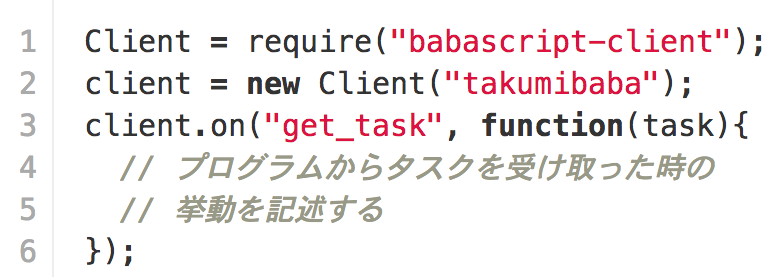
\includegraphics[width=220px]{./images/client.png}
  \caption{クライアントライブラリの基本機能 }
  \label{client}
\end{figure}

クライアントオブジェクトの宣言時、IDを指定することによって、IDに対して処理命令が発行された際にタスクを受信することができる。
また、クライアントオブジェクトが持つ ``returnValue''
メソッドを利用することで、返り値を命令発行元に返すことができる。

クライアントライブラリは、UIと完全に分離した実装となっており、かつ利用方もシンプルだ。
後述のWebアプリケーションだけでなく、様々なアプリケーションに組み込むことができる。

\subsection{Webアプリケーション}\label{webux30a2ux30d7ux30eaux30b1ux30fcux30b7ux30e7ux30f3}

BabascriptClientが得たタスクをユーザに提示するためのインタフェースとして、Webアプリケーションを実装した。
タスク情報において型指定をすることによって、ユーザに提示するUIを変化させ、型に合った返り値を選択できるようにしている。
例えば、Boolean型を指定していた場合、ユーザには true ボタンと false
ボタンが提示され、どちらかを押すと、その結果が返り値としてプログラムに返される。
また、String型を指定すれば、文字列の入力フォームとSubmitボタンが表示される。

スマートフォンに最適化したWebアプリケーションとして実装しており、様々な場面において利用可能であり、実世界におけるタスクを処理しながらでも十分に利用可能である。
図\ref{webapp-interface}のような画面を持つ。

\begin{figure}[h]
  \centering
  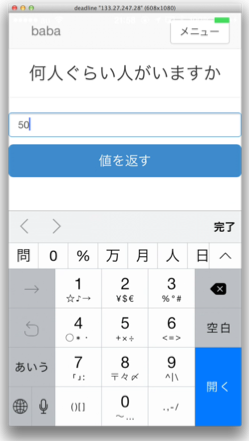
\includegraphics[width=120px]{./images/interface.png}
  \caption{Webアプリのインタフェース}
  \label{webapp-interface}
\end{figure}

\subsection{Plugin}\label{plugin}

Babascript及びBabascript
Clientに組み込むことのできるプラグイン機構を実装した。

Babascript及びBabascriptClientが発行するイベントとデータを受け取り、その都度処理を実行させることができる。
現在、以下のようなイベントが存在する

\begin{itemize}
\itemsep1pt\parskip0pt\parsep0pt
\item
  init(プラグイン読み込み時)
\item
  connect(ネットワーク接続時)
\item
  send(タスクの送信時)
\item
  receive(タスクの受信時)
\end{itemize}

具体的には、以下のようなプログラムによってプラグインを読み込むことができる

\begin{verbatim}
baba = new Babascript("baba")
baba.use(new Logger())
\end{verbatim}

具体的には、以下のようなプラグインの実装が挙げられる。

\begin{itemize}
\itemsep1pt\parskip0pt\parsep0pt
\item
  ログコレクター
\item
  データ同期
\item
  ユーザ管理
\end{itemize}

\subsection{通信と分散処理}\label{ux901aux4fe1ux3068ux5206ux6563ux51e6ux7406}

scriptとclientのタスク送受信と分散配信のために、node-linda\cite{linda}を利用した。
Websocketによる通信が行われ、リアルタイムにタスクの送受信が行われている。
script,
client共に、このnode-lindaに接続するためのライブラリを組み込んでいる。

scriptは、プログラム実行時にnode-lindaサーバに接続し、人への命令構文を実行するごとに、タスクをnode-lindaサーバに書き込む。
書き込み終了後、そのタスクと同じIDを持った返り値タスクが書き込まれるまで、node-lindaサーバの監視を行う。

clientは、プログラム起動中は常にnode-lindaサーバに接続し、指定されたIDを監視する。

\subsection{処理の流れ}\label{ux51e6ux7406ux306eux6d41ux308c}

Babascript環境は、以下のようなフローで一回の人への命令構文が実行される。

\begin{enumerate}
\def\labelenumi{\arabic{enumi}.}
\itemsep1pt\parskip0pt\parsep0pt
\item
  人への命令構文を実行する
\item
  命令構文に応じたタスクが生成される
\item
  タスクがNode-Lindaサーバを経由してクライアントへと配信される
\item
  タスクを受け取ったクライアントがユーザに処理を促す
\item
  タスク実行者が、処理結果を入力する
\item
  処理結果を元に返り値データが生成される
\item
  Node-Lindaサーバを経由して実行元プログラムに返り値が送信される
\item
  指定されたコールバック関数が実行され、処理が続く
\end{enumerate}

\subsection{実装}\label{ux5b9fux88c5}

上記システムは全てJavascriptで実装した。 Babascript
はNode.js上で動作し、 Babascript
ClientはNode.jsとWebブラウザ上で動作する。
全体図は図\ref{system}のとおりだ。

\begin{figure}[h]
  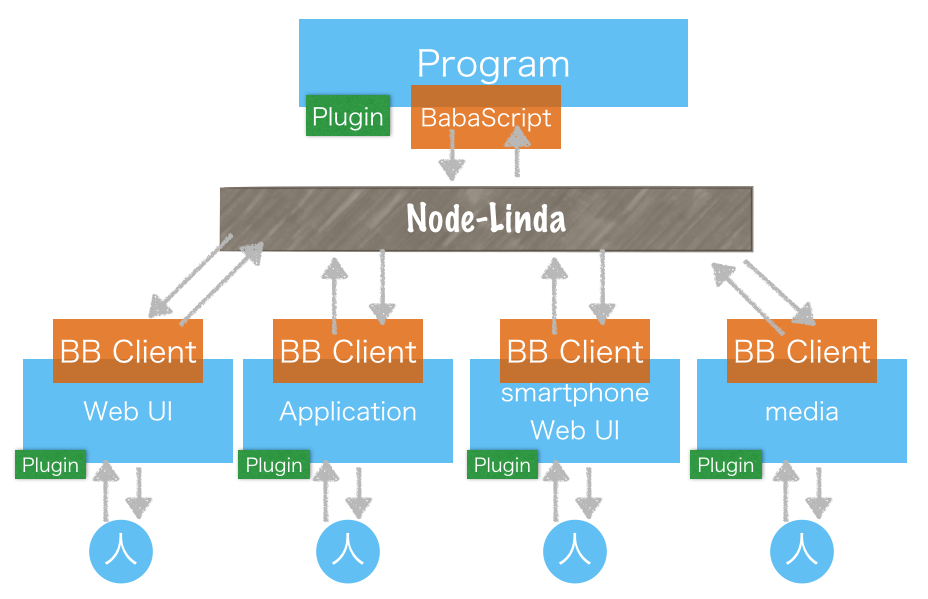
\includegraphics[width=220px]{./images/system.png}
  \caption{システム全体図}  
  \label{system}
\end{figure}

\subsubsection{タスク情報の構成}\label{ux30bfux30b9ux30afux60c5ux5831ux306eux69cbux6210}

人への処理命令構文は実行によってタスク情報を生成する。
このタスク情報は、図\ref{task}のようなjsonオブジェクトとなる。

\begin{figure}[h]
  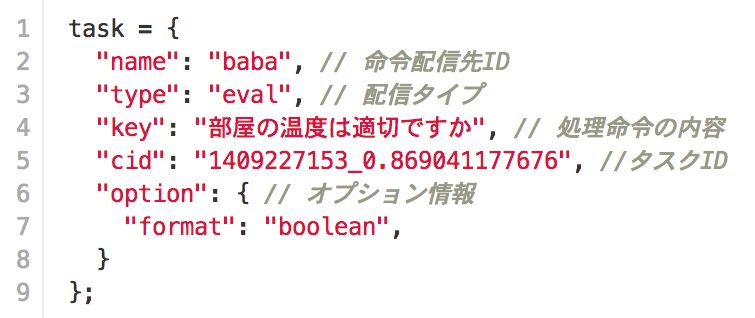
\includegraphics[width=230px]{./images/task.png}
  \caption{タスクのJSONオブジェクト}  
  \label{task}
\end{figure}

\subsubsection{実行結果の待ち方}\label{ux5b9fux884cux7d50ux679cux306eux5f85ux3061ux65b9}

人への命令構文に対する返り値が、適切に返り値として戻されるようにするために、命令ごとにユニークなIDを生成している。
ユニークIDは、人への命令構文実行時のUNIX time
と、ランダムな数値を結合した文字列である。
図\ref{task}におけるjsonオブジェクトの'cid'の項目に示されているものだ。
このユニークIDを伴った返り値が戻ってくるか、指定したタイムアウト時間に到達するか、タスクキャンセルが発生するまで、

\section{応用例}\label{ux5fdcux7528ux4f8b}

以下のような応用が考えられる。

\subsection{仕事のプログラム化}\label{ux4ed5ux4e8bux306eux30d7ux30edux30b0ux30e9ux30e0ux5316}

人への行動命令がプログラムとして記述可能になることで、人の仕事をプログラム化することができる。
プログラム化し、実行することによって、状態をプログラムによって管理することが可能となる。
つまり、条件判断や記憶が必要なことは出来るだけコンピュータ側に処理させる、といったことが可能にあんり、人は細かい条件などを覚えておいたり、自分で判断することなく、ただ指示されたことのみを実行することで、仕事を終わらせることができるようになる。
ただ指示されたことのみを実行するだけで良いならば、仕事の引き継ぎなども必要なくなり、人の代替も容易となる。

また、人同士がコミュニケーションを取ることなく、複数人を協調させるといったことも可能となる。
通常、複数人を協調させるためには、人同士が相談したり、上位の意思決定者が必要となる。
しかし、コミュニケーションはコストのかかるものであり、適切に行われない場合、問題が生じることもある。
意思決定をプログラムに委ねることによって、複数人を効率よく協調させることはとても良いと思われる。

全ての仕事をプログラム経由にすることで、詳細な実行ログや実行状況を把握することもできる。
仕事の実行量の定量化や、状況監視、状況の可視化などに活かすことができる。

\subsection{実世界プログラミング}\label{ux5b9fux4e16ux754cux30d7ux30edux30b0ux30e9ux30dfux30f3ux30b0}

人をセンサーやアクチュエータとして利用することで、人によって実世界を操作する実世界プログラミングが可能となる。
現在のセンサーやアクチュエータでは、実世界に干渉するのには限界がある。
例えば、その場の雰囲気を数値化したり文字列化するといった、コンテキスト情報を伴ったセンシングは困難である。
人というセンサーをプログラムから利用できるようにすることで、今までには実現しなかった処理が実現する。

\section{考察}\label{ux8003ux5bdf}

Babascript環境について、以下のように考察する。

\subsection{人とコンピュータの相互補完}\label{ux4ebaux3068ux30b3ux30f3ux30d4ux30e5ux30fcux30bfux306eux76f8ux4e92ux88dcux5b8c}

現状では、コンピュータは人を支援するために存在している。 しかし、

むしろ、

\subsection{処理単位としての人}\label{ux51e6ux7406ux5358ux4f4dux3068ux3057ux3066ux306eux4eba}

本研究では、人は処理を命令され実行するノードとなり、プログラム上においてコンピュータやセンサーと同等となる。
こういったことに対して心理的な拒否感を覚えることも考えられる。
しかし、一処理ノードとして扱うことによって、大きなメリットもある。
人とコンピュータ、処理に応じて適切なほうに実行させることができれば、人は人にしかできないことや人がやるべき処理にのみ集中するといったことも実現できる。
また、ただやるべきことのみを命令されて動くということは、自分で深く考えて行動する必要がないということだ。
とても楽なことでもある。

\subsection{タスク実行の遅延と実行保障性}\label{ux30bfux30b9ux30afux5b9fux884cux306eux9045ux5ef6ux3068ux5b9fux884cux4fddux969cux6027}

Babascriptによってタスク実行を依頼しても、人がすぐにタスクを実行し値を返すことを完全に保証することはできない。
タスク受信端末を見ていない、受信しても実行できないといった状況の場合、すぐに値を返すことはできない。
この際、Babascriptによる処理が原因で全体の処理が遅延する可能性がある。

また、労働関係にあるなど、タスク実行に強制力がある場合は、タスク実行が確実に行われると考えられるが、強制力がない場合はそもそもタスク受信を無視するといったことも考えられる。
タスク実行に強制力がない場合は、金銭などのインセンティブを与えるといった手段によって、実行保障性を確保するといったことが考えられる。

\subsection{例外処理}\label{ux4f8bux5916ux51e6ux7406}

Babascript環境において、命令文と現実との乖離によって適切な返り値を選択・記述ができなくなるといった可能性がある。
これは、現実が刻々と変化していることなどから、完全に避ける事の出来ない問題であると考える。
この際、無理やり値を返すといった処理をしてしまうと、本来の状態とは違った判断がなされてしまう危険性がある。
命令文とは明らかに現実が異なっている場合などは、タスク実行者から例外としてプログラムに通知出来るような仕組みの実装によって、問題の解決へと繋げられると考える。

\subsection{命令内容の粒度}\label{ux547dux4ee4ux5185ux5bb9ux306eux7c92ux5ea6}

Babascriptでは、タスクの命令文の記述には制限がないため、自由となっている。
抽象度が高すぎる命令は、あいまいな表記となり、タスク実行者にとって理解しづらい文面となり得る。
その結果、想定外の処理が実行され、意図しない結果を招く恐れがある。
抽象度が低すぎる命令は、全体の処理内容にもよるが、プログラム自体が冗長となり得る。
プログラムとタスク実行者の間のやりとりが増え、通信や待機時間などがボトルネックとなる可能性がある。
また、タスク実行者にとっても、やりとりが増えることで負担増になると考えられる。
処理ごとに異なると考えられるが、命令文は適切な抽象度に設計しなくてはならない。

\subsection{複数命令の同時実行}\label{ux8907ux6570ux547dux4ee4ux306eux540cux6642ux5b9fux884c}

複数のプログラムから同時に一人のタスク実行者へとタスクが配信される可能性がある。
この際、異なるコンテキストにある命令が交互に配信され、タスク実行に大きな障害をもたらす可能性がある。
例えば、料理プログラムと掃除プログラムが同時に実行された場合、鍋で煮ている途中で「洗剤を投入しろ」などといった命令が配信されることが考えられる。

この問題は、全てのBabascriptプログラム中において、一人のタスク実行者は一つのプログラムからのみ、連続してタスクを受信できるような仕組みを用意することによって、解決可能であると考えられる。
また、応用アプリケーションでの実装になるが、コンテキストを明示し、どの処理系におけるタスクなのかをタスク実行者に示すといった手段によっても解決可能である。

\section{関連研究}\label{ux95a2ux9023ux7814ux7a76}

計算機では処理が難しいようなタスクを解決するために、人を計算資源として利用する手法はヒューマンコンピュテーション\cite{HumanComputation}と呼ばれ、様々な研究が行われている。
インターネットを介して不特定多数の群衆にタスクを実行させるクラウドソーシングと組み合わせた研究事例も多く存在する。
クラウドソーシングのプラットフォームとしては、Amazon Mechanical
Turk\cite{mechanicalturk}が存在する。 Barowy
らは、CrowdProgrammingという概念を提唱し、プログラミング言語内においてクラウドソーシングによる計算とコンピュータによる計算の統合を実現した\cite{automan}。
Franklin
らは、機械だけでは答えられないようなDBへのクエリに対する応答を、クラウドソーシングを用いることで返答可能にするCrowdDBを提案している\cite{crowddb}。
Morishima
らは、人をデータソースとしてプログラムの中で利用する手法を提案している\cite{cylog}。
jabberwocky crowdforge
これらの研究では、クラウドソーシングを利用した問題解決手法の提案をしている。
本研究は、不特定多数の群衆をプログラムするためのものではなく、実世界の操作なども含むため、家族や職場の人のような特定可能な人物を対象としている。
また、人を計算資源やデータソースとしてシステムに組み込むことを前提としているが、本研究は、計算資源やデータソースに限らず、実世界への干渉等も対象としている。
本研究はより汎用的な枠組みであると言える。

ユビキタスコンピューティングの研究分野においては、Human as
Sensorという概念も提唱されている。
PRISMは、スマートフォンを利用したセンシングプラットフォームだ\cite{prism}。
Liuらは、ソーシャルメディア上の人をセンサーとして扱ったQ\&AサービスMoboQを提案し、その検証を行った。
Human as
Sensorに類する研究では、人をセンサーとして扱うことを対象としているが、本研究ではセンサーのみを対象としていない。

Chengらは、モーションプラットフォームにおけるモーターやメカニカル機構の代替として人を利用したHaptic
Turkを提案している\cite{hapticturk}。 Haptic
Turkはゲームでの利用に特化したものだ。
本研究は、用途を限らない汎用的な仕組みとなっている。

加藤らは、人とロボット間でのタスク共有システム
Sharedoを提案した\cite{sharedo}。
人とロボットのタスク実行における協調は、本研究の主眼である「何かの処理を実現するとき、人とコンピュータは相補的に動作するべき」という考えと大きく類似している。

\section{おわりに}\label{ux304aux308fux308aux306b}

本論文では、人への命令構文をプログラムに付与可能なプログラミング環境Babascriptを提案した。
Babascript環境においては、プログラム上において人は、コンピュータと同じ処理ノードとして存在し、関数実行によって処理内容を受け取り、実行・値を返す存在になれる。
これによって、プログラマブルになりつつある世界において人自身もその一部になることが可能となる。

また、Babascript環境によって実現する応用例を示すことによって、人をプログラマブルにした際のメリットを示した。

今後は、議論で述べたBabascriptの問題点などを改善していく。
